\chapter{Indexation par termes-clés en domaines de spécialités}
\label{chap:main-domain_specific_keyphrase_annotation}
  \chaptercite{
    La multiplication des bases de données et l'information devenue
    \og{}marché\fg{} (donc rentable) ont entraîné d'autres corps de métiers à
    s'intéresser à la pratique de l'indexation. Mais ce sont les bibliothécaires
    et documentalistes qui en ont défini les méthodes, les usages et les outils.
  }{
    \newcite{guinchat1996techniquesdocumentaires}
  }

  %-----------------------------------------------------------------------------

  \section{Introduction}
  \label{sec:main:domain_specific_keyphrase_annotation-introduction}
    Dans ce chapitre, nous nous interessons à l'indexation par
    termes-clés en domaines de spécialités. Dans la littérature, l'indexation
    par termes-clés se divise en deux catégories~: l'extraction de termes-clés,
    qui fournit des termes-clés apparaissant dans le contenu du document, et
    l'assignement de termes-clés, qui fournit des termes-clés appartenant à un
    vocabulaire contrôlé et n'apparaissant pas nécessairement dans le document.
    Alors que l'indexation par termes-clés est principalement réalisée au seul
    moyen de l'extraction de termes-clés, nous montrons que l'assignement de
    termes-clés joue un rôle important en domaines de spécialités.

    Dans ce chapitre, nous décrivons le comportement des indexeurs
    professionnels d'une bibliothèque numérique (Inist), puis nous proposons une
    automatisation de ce comportement. Les indexeurs professionnels assignent à
    chaque document des termes-clés du domaine, répertoriés dans un vocabulaire
    contrôlé, et extraient des termes-clés hors du vocabulaire contrôlé
    lorsqu'ils sont très spécifiques au document ou lorsqu'il s'agit de nouveaux
    concepts. Pour reproduire ce comportement, nous étendons nos travaux
    précédents par l'intégration, dans le graphe de sujets, des termes-clés du
    domaine, c'est-à-dire du vocabulaire contrôlé. Ce dernier n'étant cependant
    pas disponible dans tous les cas de figure, nous en déterminons une
    approximation à partir des termes-clés de référence des données
    d'entraînement.

    Enfin, nous présentons les premiers résultats d'une évaluation manuelle de
    nos travaux en domaines de spécialités. Pour cette évaluation, nous
    proposons un protocole et des metriques permettant d'évaluer deux aspects.
    L'un permet d'évaluer la performance d'une méthode d'après la pertinence des
    termes-clés qu'elle extrait/assigne et l'autre permet d'évaluer la
    performance d'une méthode en terme de quantité d'information importante
    capturée par ces termes-clés.

  %-----------------------------------------------------------------------------

  \section[Indexation manuelle dans le contexte d'une bibliothèque scientifique]{Indexation manuelle dans le contexte d'une bibliothèque\\scientifique}
  \label{sec:main-domain_specific_keyphrase_annotation-manual_keyphrase_annotation}
    Dans cette section, nous présentons la tâche d'indexation par termes-clés
    réalisée manuellement au sein d'un organisme gestionnaire d'une bibliothèque
    scientifique. Pour cela, nous nous fondons sur les propos recueillis des
    indexeurs professionnels de l'Inist, dont les données Termith sont issues.
    La bibliothèque numérique scientifique de l'Inist est indexée à l'aide de
    termes-clés majoritairement issus de ressources terminologique définies et
    maintenues par les indexeurs.

    \subsection{Principes généraux}
    \label{subsec:main-domain_specific_keyphrase_annotation-manual_keyphrase_annotation-principles}
      L'indexation manuelle à l'Inist est régie par cinq pilliers~:
      \begin{enumerate}
        \item{Conformité~: les termes-clés doivent être conformes au contenu du
              document et au langage documentaire utilisé dans son domaine~;}
        \item{Exhaustivité~: les termes-clés doivent représenter tous les
              aspects importants du document, même lorsque ceux-ci sont
              implicites~;}
        \item{Homogénéité~: les termes-clés des documents d'un même domaine
              doivent être cohérents et identiques lorsqu'ils représentent le
              même concept~;}
        \item{Spécificité~: les termes-clés doivent décrire le contenu d'un
              document au niveau le plus spécifique du document et peuvent
              parfois être accompagnés de termes-clés plus génériques afin de
              restituer le contenu du document dans son domaine~;}
        \item{Impartialité~: les termes-clés ne doivent pas être représentatif
              d'un jugement apporté par l'indexeur.}
      \end{enumerate}
      Ces cinq pilliers font écho à des principes que nous retrouvons aussi bien
      en extraction et en assignement automatique de termes-clés. Les trois
      premiers pilliers impliquent une indexation majoritairement contrôlée,
      comme en assignement automatique de termes-clés, et le quatrième pillier
      implique une indexation en partie libre, comme en extraction de
      termes-clés.

      Ces principes généraux de l'indexation manuelle par termes-clés remettent
      en cause la séparation entre extraction et assignement de termes-clés dans
      le contexte de l'indexation automatique en domaines de spécialités. En
      effet, une indexation par termes-clés à un niveau professionnel se doit de
      respecter le langage de spécialité employé dans le domaine des documents
      indexés (assignement), mais elle se doit aussi d'être exhaustive et donc
      de fournir des termes-clés très spécifiques, voir de nouveaux
      concepts (extraction).

    \subsection{Ressources}
    \label{subsec:main-domain_specific_keyphrase_annotation-manual_keyphrase_annotation-resources}
      L'indexation par termes-clés réalisée par les indexeurs professionnels de
      l'Inist s'appuie sur plusieurs ressources. Ces dernières sont
      représentatives d'une expertise de terrain dans chaque domaine de
      spécialité (grille d'indexation), d'une expertise terminologique
      (vocabulaire contrôlé) et d'une expertise documentaire (règles de
      préindexation).

      \subsubsection{Grille d'indexation}
      \label{subsubsec:main-domain_specific_keyphrase_annotation-manual_keyphrase_annotation-resources-indexing_guidelines}
        La grille d'indexation est un guide qui indique les notions qui peuvent
        être pertinentes à indexer selon le domaine de spécialité et la
        problématique du document. Elle peut-être assimilée à un formulaire à
        compléter pour chaque document (cf tableau~\ref{fig:indexing_grid}). La
        grille d'indexation est un canevas donné à titre indicatif aux
        indexeurs. Ces derniers sont les seuls juges pour décider si elle est
        adaptée ou non pour indexer un document.
        \begin{table}[h!]
          \centering
          \begin{tabular}{l|l}
            \toprule
            \textbf{Champ} & \textbf{Exemple}\\
            \hline
            Domaine & enseignement des langues~; linguistique appliquée\\
            Environnement & langue scientifique~; langue de spécialité~; discours scientifique\\
            Objet d'étude & argumentation~; réthorique~; article de recherche\\
            \bottomrule
          \end{tabular}
          \caption[
            Exemple de remplissage de la grille d'indexation de linguistique
          ]{
            Exemple de remplissage de la grille d'indexation de linguistique,
            pour la notice présentée dans la figure \TODO{???} (page
            \TODO{???}) \REMARK{Attention, l'exemple va changer}
            \label{fig:indexing_grid}
          }
        \end{table}

      \subsubsection{Vocabulaire contrôlé}
      \label{subsubsec:main-domain_specific_keyphrase_annotation-manual_keyphrase_annotation-resources-controlled_vocabulary}
        Le vocabulaire contrôlé est un lexique qui recense et organise les
        termes d'un domaine de spécialité. Dans le contexte de l'indexation par
        termes-clés, il définit le langage documentaire à utiliser pour les
        termes-clés. C'est la ressource indispensable pour assurer la conformité
        et l'homogénéité de l'indexation. Il doit toutefois être mis à jour
        régulièrement, soit par une veille terminologique, soit au fur et à
        mesure des indexations manuelles.

      \subsubsection{Règles de préindexation}
      \label{subsubsec:main-domain_specific_keyphrase_annotation-manual_keyphrase_annotation-resources-preindexing_rules}
        Les règles de préindexation sont des règles qui définissent les
        termes-clés du vocabulaire contrôlé à assigner en fonction soit (1)
        d'une unité textuelle qui occure dans le document (\TODO{exemple}), soit
        (2) d'un terme-clé assigné au document (\TODO{exemple}). Fortement
        couplées avec le vocabulaire contrôlé, les règles de préindexation
        permettent d'assurer la conformité et l'homogénéité de l'indexation.
        Elles contribuent aussi a l'exhaustivité, en permettant l'assignement
        d'aspects implicites dans le document (1), et à la spécificité, en
        restituant le contenu du document dans son domaine grâce au termes-clés
        génériques (2).

    \subsection{Méthodologie}
    \label{subsec:main-domain_specific_keyphrase_annotation-manual_keyphrase_annotation-methodology}
      Nous distinguons cinq phases lors de l'indexation manuelle par
      termes-clés~:
      \begin{enumerate}
        \item{Choix des ressources à utiliser (grille d'indexation, vocabulaire
              contrôlé et règles de préindexation)~;}
        \item{Utilisation d'un système automatisé de proposition de termes-clés
              à partir des règles de préindexation~;}
        \item{Assignement de termes-clés respectant le langage documentaire
              (dans le vocabulaire contrôlé)~;}
        \item{Assignement de termes-clés génériques afin de replacer les
              termes-clés trop spécifiques dans leur domaine~;}
        \item{Extraction des termes-clés ne respectant pas le langage
              documentaire mais utiles pour décrire le contenu le plus important
              du document.}
      \end{enumerate}

      L'indexation Inist peut être qualifiée de semi-automatique. En effet, la
      deuxième phase est automatisée et systématiquement validée par l'indexeur,
      de sorte à réduire le temps d'indexation et à minimiser les oublis de la
      part de l'indexeur. Cette phase montre la prise de conscience, dans les
      organismes gestionnaires de bibliothèques scientifiques, que l'indexation
      est une tâche difficile et coûteuse à entreprendre manuellement.
      Toutefois, en croisant l'étude bibliographique réalisée dans le
      chapitre~\ref{chap:main-state_of_the_art}
      (page~\pageref{chap:main-state_of_the_art}), nous nous apercevons
      qu'aucune méthode ne répond actuellement à leurs besoins.

    \subsection{Bilan}
    \label{subsec:main-domain_specific_keyphrase_annotation-manual_keyphrase_annotation-conclusion}
      L'indexation manuelle en domaines de spécialités que nous avons présenté
      suit des principes d'indexation que nous retrouvons soit en extraction,
      soit en assignement. Alors qu'en indexation automatique par termes-clés,
      les méthodes d'extraction prédominent sur les méthodes d'assignement,
      notre étude de l'indexation réalisée par des indexeurs professionnels
      montre que l'assignement est la pratique préférée, car elle assure
      conformité, exhaustivité et homogénéité, et que l'extraction doit
      uniquement servir à la compléter. Nous observons une tentative d'ouverture
      des organismes de gestion de bibliothèques numériques vers une indexation
      automatique par termes-clés, mais aucune méthode ne répond actuellement à
      leurs besoins très spécifiques.

  %-----------------------------------------------------------------------------

  \section{Indexation automatique en domaines de spécialités}
  \label{sec:main-domain_specific_keyphrase_annotation-supervised_automatic_keyphrase_extraction}
    Cette section introduit TopicCoRank, une extension supervisée de TopicRank
    adaptée à l'indexation par termes-clés en domaines de spécialités. En nous
    fondant sur l'indexation réalisée par des indexeurs professionnels présentée
    précédemment, nous ajoutons à TopicRank la capacité à assigner des
    termes-clés qui ne cooccurrent pas nécessairement dans le document et qui
    respectent le langage documentaire. Pour cela, nous approximons un
    vocabulaire contrôlé à partir des termes-clés de référence des données
    d'entraînement. Nous assurons autant que possible l'homogénéité de
    l'assignement en déterminant conjointement l'importance des sujets du
    document et des termes-clés de référence du domaine~: les sujets importants
    du documents influencent l'importance des termes-clés de référence et ces
    derniers influencent l'importance des sujets du document.

    \subsection{TopicCoRank}
    \label{subsec:main-domain_specific_keyphrase_annotation-supervised_automatic_keyphrase_annotation-topiccorank}
      TopicCoRank est une méthode supervisée à base de graphe qui réalise
      simultanément extraction et assignement de termes-clés. Issue de
      TopicRank, elle en modifie les étapes suivantes~: construction du graphe,
      ordonnancement et sélection des termes-clés. La construction du graphe
      étend le graphe de sujet initial de TopicRank en l'unifiant à un graphe
      représentatif des termes-clés de référence du domaine~; l'ordonnancement
      est désormais conjoint pour les sujets du document et les termes-clés de
      référence du domaine~; la sélection des termes-clés ajoute la possibilité
      d'assigner en puisant dans le graphe représentatif des termes-clés du
      domaine.
      
      L'identification des sujets reste inchangée. L'évaluation de TopicRank en
      domaines de spécialités ayant montré de meilleures performances lorsque
      les termes-clés candidats sont sélectionnés par notre méthode de sélection
      (\textsc{Lr-Np}), TopicCoRank utilise cette dernière.

      \subsubsection{Construction du graphe}
      \label{subsubsec:main-domain_specific_keyphrase_annotation-supervised_automatic_keyphrase_extraction-topiccorank-graph_construction}
        Afin de réaliser simultanément extraction et assignement de termes-clés,
        TopicCoRank unifie deux graphes représentant le document (graphe de
        sujets) et les termes-clés de son domaine (graphe du domaine). Ce
        dernier graphe est construit à partir des termes-clés de référence des
        documents d'entraînement fournis avec une collection de données. Comme
        \newcite{chaimongkol2013technicaltermextraction} l'ont fait avant nous
        pour l'extraction de termes techniques, nous faisons l'hypothèse que les
        termes-clés de référence des documents d'entraînement constituent la
        terminologie du domaine et nous les utilisons comme substitut au
        vocabulaire contrôlé. Contrairement aux termes-clés candidats
        sélectionnés dans le document, les termes-clés de référence ne sont pas
        jugés redondants\footnote{Cette hypothèse est d'autant plus forte que
        les données d'entraînement sont issues d'une indexation établie dans un
        contexte professionnel. Elle l'est moins pour les autres données.}.
        TopicCoRank ne les groupe pas avant de construire le graphe du domaine.

        Soit le graphe unifié non orienté $G = (N, A =
        A_{\textnormal{\textit{interne}}} \cup
        A_{\textnormal{\textit{externe}}})$. $N$ dénote indifféremment les
        sujets et les termes-clés de référence. $A$ regroupe les arêtes
        $A_{\textnormal{\textit{interne}}}$, qui connectent deux sujets ou deux
        termes-clés de référence, et les arêtes
        $A_{\textnormal{\textit{externe}}}$, qui connectent un sujet à un
        terme-clé de référence (cf. figure~\ref{fig:topiccorank_graph}). Le
        graphe de sujets et le graphe du domaine sont unifiés grâce aux arêtes
        $A_{\textnormal{\textit{externe}}}$. Une arête
        $A_{\textnormal{\textit{externe}}}$ est ajoutée pour connecter un sujet
        et un terme-clé de référence si, et seulement si, le terme-clé fait
        partie des termes-clés candidats qui composent le sujet
        (\TODO{exemple}). En d'autres termes, TopicCoRank considère le domaine
        comme une carte conceptuelle et connecte le document au domaine par
        l'intermédiaire des concepts qu'ils partagent.
        \begin{figure}
          \newcommand{\xslant}{0.25}
          \newcommand{\yslant}{0}

          \centering
          \begin{tikzpicture}[transform shape, scale=.75]
            % frame
            \node [draw,
                   rectangle,
                   minimum width=.7\linewidth,
                   minimum height=8em,
                   xslant=\xslant,
                   yslant=\yslant] (domain_graph) {};
            \node [above=of domain_graph,
                   xshift=.36\linewidth,
                   yshift=8em,
                   anchor=south east] (domain_graph_label) {termes-clés de référence};

            \node [draw,
                   circle,
                   above=of domain_graph,
                   xshift=.3\linewidth,
                 yshift=5em] (domain_node1) {$V_1$};
            \node [draw,
                   circle,
                   above=of domain_graph,
                   xshift=-.3\linewidth,
                   yshift=5em] (domain_node2) {$V_2$};
            \node [draw,
                   circle,
                   above=of domain_graph,
                   yshift=5em] (domain_node3) {$V_3$};
            \node [draw,
                   circle,
                   above=of domain_graph,
                   xshift=.15\linewidth,
                   yshift=.75em] (domain_node4) {$V_4$};
            \node [draw,
                   circle,
                   above=of domain_graph,
                   xshift=-.15\linewidth,
                   yshift=.75em] (domain_node5) {$V_5$};

            \draw (domain_node1) -- (domain_node3);
            \draw (domain_node2) -- (domain_node3);
            \draw (domain_node2) -- (domain_node4);
            \draw (domain_node4) -- (domain_node5);
            \draw (domain_node4) -- (domain_node3);

            % document
            \node [draw,
                   rectangle,
                   minimum width=.7\linewidth,
                   minimum height=8em,
                   xslant=\xslant,
                   yslant=\yslant,
                   above=of domain_graph,
                   xshift=-2em] (document_graph) {};
            \node [below=of document_graph,
                   xshift=-.36\linewidth,
                   yshift=-8em,
                   anchor=north west] (document_graph_label) {sujets du document};

            \node [draw,
                   circle,
                   regular polygon sides=8,
                   below=of document_graph,
                   xshift=.3\linewidth,
                   yshift=-5em] (document_node1) {$V_6$};
            \node [draw,
                   circle,
                   regular polygon sides=8,
                   below=of document_graph,
                   xshift=-.3\linewidth,
                   yshift=-5em] (document_node2) {$V_7$};
            \node [draw,
                   circle,
                   regular polygon sides=8,
                   below=of document_graph,
                 yshift=-5em] (document_node3) {$V_8$};
            \node [draw,
                   circle,
                   regular polygon sides=8,
                   below=of document_graph,
                   xshift=.15\linewidth,
                   yshift=-.75em] (document_node4) {$V_9$};

            \draw (document_node2) -- (document_node3);
            \draw (document_node3) -- (document_node1);
            \draw (document_node1) -- (document_node4);
            \draw (document_node3) -- (document_node4);

            % extra link
            \draw [dashed] (document_node2) -- (domain_node2);
            \draw [dashed] (document_node3) -- (domain_node3);
            \draw [dashed] (document_node4) -- (domain_node1);
            \draw [dashed] (document_node3) -- (domain_node4);

            % legend
            \node [right=of document_graph, xshift=2em, yshift=-9.25em] (legend_title) {\underline{Légende~:}};
            \node [below=of legend_title, xshift=-1em, yshift=2em] (begin_inner) {};
            \node [right=of begin_inner] (end_inner) {: $A_\textnormal{\textit{interne}}$};
            \node [below=of begin_inner, yshift=1.5em] (begin_outer) {};
            \node [right=of begin_outer] (end_outer) {: $A_\textnormal{\textit{externe}}$};

            \draw (legend_title.north  -| end_outer.east) rectangle (end_outer.south -| legend_title.west);

            \draw (begin_inner) -- (end_inner);
            \draw [dashed] (begin_outer) -- (end_outer);
          \end{tikzpicture}
          \caption{Illustration du graphe unifié utilisé par TopicCoRank
                   \label{fig:topiccorank_graph}}
        \end{figure}

        Pour permettre un ordonnancement conjoint des sujets et des termes-clés
        de référence, le schéma de connexion entre deux sujets et entre deux
        termes-clés de référence (arêtes $A_\textnormal{\textit{interne}}$) doit
        être homogénéisé. En effet, si les conditions de connexion et si la
        pondération des arêtes ne sont pas, respectivement, sémantiquement
        équivalentes et du même ordre de grandeur, alors l'impact du domaine sur
        le document, et inversement, sera marginal et inexploitable. Pour
        obtenir un graphe unifié homogène, TopicCoRank connecte deux sujets ou
        deux termes-clés de référence $n_i$ et $n_j$ lorsqu'ils apparaissent
        dans le même contexte et pondère leur arête par le nombre de fois que
        cela se produit ($\textnormal{poids}(n_i, n_j)$), normalisé par le
        nombre total de contextes. Lorsqu'il s'agit des sujets, le contexte est
        une phrase du document (\TODO{exemple})~; lorsqu'il s'agit des
        termes-clés de référence, le contexte est l'ensemble des termes-clés de
        référence d'un document d'entraînement (\TODO{exemple}). Les contextes
        étant utilisés pour la création du graphe, le graphe de sujets n'est
        plus complet comme pour TopicRank. Il n'y a  cependant pas de fenêtre de
        cooccurrences fixée à une valeur prédéfinie, car c'est la phrase.

      \subsubsection{Ordonnancement conjoint des sujets et des termes-clés de référence}
      \label{subsubsec:main-domain_specific_keyphrase_annotation-supervised_automatic_keyphrase_extraction-topiccorank-co_ranking}
        L'ordonnancement conjoint des sujets et des termes-clés de référence
        établit l'ordre d'importance des sujets du document et des termes-clés
        de référence du domaine vis-à-vis du contenu du document. Le score
        d'importance attribué aux sujets et aux termes-clés de référence est
        obtenu avec le même algorithme et la même instance de cet algorithme.
        L'ordonnancement fournit une seule liste ordonnée, mêlant sujets et
        termes-clés de référence.

        TopicCoRank reprend le principe de la recommandation de TopicRank et
        l'adapte au problème d'ordonnancement conjoint. Les premières hypothèses
        de recommandation sont donc les mêmes que celle de TopicRank~:
        \begin{itemize}
          \item{un sujet est d'autant plus important s'il est fortement connecté
                à un grand nombre de sujets et si les sujets avec lesquels il
                est fortement connecté sont importants~;}
          \item{un terme-clé de référence est d'autant plus important s'il est
                fortement connecté à un grand nombre de termes-clés de référence
                et si les termes-clés de référence avec lesquels il est connecté
                sont importants.}
        \end{itemize}
        Ces hypothèses de recommandation, que nous qualifions d'internes,
        permettent d'établir l'importance des sujets les uns par rapport aux
        autres et l'importance des termes-clés de référence les uns par rapport
        aux autres. Cependant, elles ne permettent pas de tirer profit des
        termes-clés de référence importants pour renforcer l'importance des
        sujets qui y sont connectés, et inversement. De plus,
        l'importance des termes-clés de référence est indépendante du document
        et, pour la même collection de données, l'importance des termes-clés de
        référence est toujours la même quelque soit le document. Nous ajoutons
        donc deux nouvelles hypothèses de recommandation, que nous qualifions
        d'externes~:
        \begin{itemize}
          \item{un sujet est d'autant plus important s'il est représenté par des
                termes-clés de référence importants~;}
          \item{un terme-clé de référence est d'autant plus important vis-à-vis
                du contenu du document s'il est connecté à l'un de ses sujets
                importants.}
        \end{itemize}
        Sujets et termes-clés de référence sont ainsi évalués d'après leur usage
        dans le document et leur importance dans le domaine. L'ordonnancement
        des uns joue un rôle sur celui des autres et permet ainsi d'effectuer
        conjointement extraction et assignement.

        Mathématiquement, la formule d'ordonnancement de TopicRank est adaptée
        en préservant la recommandation interne
        ($R_{\textnormal{\textit{interne}}}$) et en remplaçant l'aléa
        $(1 - \lambda)$ par la recommandation externe
        ($R_{\textnormal{\textit{externe}}}$)~:
        \TODO{il faut s'assurer que l'aléa et ce qu'il représente est bien
        introduit dans l'état de l'art et/ou TopicRank}
        \begin{align}
          S(n_i) &= (1 - \lambda)\ R_{\textnormal{\textit{externe}}}(n_i) + \lambda\ R_{\textnormal{\textit{interne}}}(n_i)\label{math:topiccorank}\\
          R_{\textnormal{\textit{interne}}}(n_i) &= \sum_{n_j \in A_{\textnormal{\textit{interne}}}(n_i)}{\frac{\textnormal{poids}(n_j, n_i) \times S(n_j)}{\mathlarger\sum_{n_k \in A_{\textnormal{\textit{interne}}}(n_j)}{{\textnormal{poids}(n_j, n_k)}}}}\label{math:rin}\\
          R_{\textnormal{\textit{externe}}}(n_i) &= \sum_{n_j \in A_{\textnormal{\textit{externe}}}(n_i)}{\frac{S(n_j)}{|A_{\textnormal{\textit{externe}}}(n_j)|}}\label{math:rout}
        \end{align}
        où $A_{\textnormal{\textit{interne}}}(n_i)$ représente l'ensemble de
        tous les n\oe{}uds connectés au n\oe{}ud $n_i$ par une arête
        $A_\textnormal{\textit{interne}}$, où
        $A_{\textnormal{\textit{externe}}}(n_i)$ représente l'ensemble de tous
        les n\oe{}uds connectés au n\oe{}ud $n_i$ par une arête
        $A_\textnormal{\textit{externe}}$ et où le facteur $\lambda$ permet
        désormais de définir la recommandation la plus influente entre
        $R_{\textnormal{\textit{interne}}}$ et
        $R_{\textnormal{\textit{externe}}}$. Par défaut, nous définissons
        $\lambda=0,5$ afin de donner autant de poids aux deux recommandations.

      \subsubsection{Sélection des termes-clés}
      \label{subsubsec:main-domain_specific_keyphrase_annotation-supervised_automatic_keyphrase_extraction-topiccorank-keyphrase_selection}
        Pour terminer l'indexation par termes-clés, TopicCoRank utilise l'ordre
        d'importance $S$ des sujets et termes-clés de référence pour déterminer
        les termes-clés du document. Les $k$ n\oe{}uds du graphe unifié ayant
        obtenu les meilleurs scores sont retenus, qu'ils soient des sujets ou
        des termes-clés de référence.

        Lorsqu'un termes-clés de référence doit être assigné, une étape de
        vérification supplémentaire est effectuée pour s'assurer que son
        importance calculée relève aussi bien du domaine que du document. En
        effet, il est possible que le graphe du domaine soit constitué de
        composantes connexes, soit de sous-graphes dont les n\oe{}uds ne sont
        connectés qu'entre eux. Dans ce cas, il est possible qu'un terme-clé de
        référence d'un sous-graphe ne soit connecté ni directement ni
        indirectement (par l'intermédiaire d'un autre n\oe{}uds) à un sujet du
        document. Son importance est donc déterminée uniquement à partir du
        domaine et il n'est donc pas pertinent de l'assigner au document.

        Lorsque un n\oe{}ud retenu représente un sujet, c'est la même stratégie
        que celle de TopicRank qui est appliquée. Pour un sujet donné, le
        terme-clé extrait est son terme-clé candidat qui apparaît en premier
        dans le document.

      \subsubsection{Exemple}
      \label{subsubsec:main-domain_specific_keyphrase_annotation-supervised_automatic_keyphrase_extraction-topiccorank-exemple}
        \TODO{\dots}

    \subsection{Évaluation}
    \label{subsec:main-domain_specific_keyphrase_annotation-supervised_automatic_keyphrase_annotation-evaluation}
      Pour valider notre approche, nous réalisons deux séries d'expériences.
      Dans un premier temps, nous comparons TopicCoRank à plusieurs méthodes de
      référence et analysons son comportement en domaine de spécialité, donc sur
      les collections Termith. Dans un second temps, nous étudions l'application
      de TopicCoRank dans le cas général sur les collections \textsc{De}ft,
      SemEval et \textsc{Duc}\footnote{Constituées de documents scientifiques,
      les ressources \textsc{De}ft et SemEval peuvent aussi être considérées
      commes des données en domaines de spécialités. Cependant, elles regroupent
      des documents de sous-disciplines très éloignées et leurs termes-clés
      n'ont pas été annotés avec la rigueur documentaire.}.

      \subsubsection{Méthodes de référence}
      \label{subsubsec:main-domain_specific_keyphrase_annotation-supervised_automatic_keyphrase_annotation-evaluation-baselines}
        Dans nos expériences, nous comparons TopicCoRank à \textsc{Tf-Idf},
        TopicRank et \textsc{Kea++}. Pour cette dernière, nous utilisons les
        thésaurus décrivant les vocabulaires contrôlés de l'Inist en
        linguistique, sciences de l'information, archéologie et chimie. Pour les
        ressources autres que Termith, nous ne disposons pas de vocabulaires
        contrôlés adéquats et n'appliquons donc pas \textsc{Kea++}.

        Nous comparons aussi TopicCoRank à deux variantes. La première,
        TopicCoRank$_\textnormal{\textit{extr.}}$, ne réalise que l'extraction
        de termes-clés~; la seconde,
        TopicCoRank$_\textnormal{\textit{assign.}}$, n'effectue que
        l'assignement.

      \subsubsection{Collections de données}
      \label{subsubsec:main-domain_specific_keyphrase_annotation-supervised_automatic_keyphrase_annotation-evaluation-evaluation_data}
        Nous utilisons les collections Termith pour l'évaluation en domaines de
        spécialités et les collections \textsc{De}ft, SemEval et \textsc{Duc}
        pour l'évaluation dans le cas général.
        
        Pour \textsc{Duc}, qui n'est pas divisé en ensembles d'entraînement et
        de test, nous tirons partie des 30 sujets d'actualité répertoriés en
        construisant un graphe \og{}de domaine\fg{} unique pour chaque document
        à partir des autres documents du même sujet d'actualité.
        
        Pour SemEval, nous construisons quatre graphes de domaine à partir des
        documents d'entraînement des quatre catégories \textsc{Acm} (C2.4, H3.3,
        I2.11 et J4) et utilisons l'un ou l'autre de ces graphes selon la
        catégorie du document de test. 
      
      \subsubsection{Mesures d'évaluation}
      \label{subsubsec:main-domain_specific_keyphrase_annotation-supervised_automatic_keyphrase_annotation-evaluation-evaluation_measures}
        Les performances des méthodes d'extraction de termes-clés sont exprimées
        en termes de précision (P), rappel (R) et f-mesure (f1-mesure, F). En
        accord avec l'évaluation menée dans les travaux précédents, nous
        considérons correcte l'extraction d'une variante flexionnelle d'un
        terme-clé de référence~\cite{kim2010semeval}. Les opérations de
        comparaison entre les termes-clés de référence et les termes-clés
        extraits sont donc effectuées à partir de la racine des mots qui les
        composent. Pour cela, nous utilisons la méthode de
        \newcite{porter1980suffixstripping}.

        Nous représentons aussi les résultats sous la forme de courbes de
        rappel--précision. Celles-ci permettent d'observer si une méthode domine
        les autres pour les critères de rappel et de précision. En optimisation
        multi-critères, nous parlons de front de Pareto optimal, c'est à dire de
        la méthode pour laquelle aucune autre méthode n'obtient de meilleures
        performances. Pour générer ces courbes, nous calculons la précision et
        le rappel lorsque  le nombre de termes-clés extraits/assignés varie de
        un jusqu'au nombre total de termes-clés
        candidats~\cite{hassan2010conundrums}.
      
      \subsubsection{Évaluation de TopicCoRank en domaines de spécialités}
      \label{subsubsec:main-domain_specific_keyphrase_annotation-supervised_automatic_keyphrase_annotation-evaluation-topiccorank_specific_domains}
        \TODO{intro.}

        Le tableau~\ref{tab:topiccorank-comparison_results_termith} montre les
        performances de TopicCoRank en domaines de spécialités (linguistique,
        sciences de l'information, archéologie, chimie) comparées à celles des
        méthodes de référence. Globalement, les résultats montrent l'apport
        d'ordonner conjointement les sujets du document et les termes-clés de
        référence du domaine pour extraire et/ou assigner des termes-clés. En
        domaines de spécialités, c'est la variante de TopicCoRank réalisant
        uniquement l'assignement (TopicCoRank$_\textnormal{assign.}$) qui est la
        plus performante, suivie par TopicCoRank,
        TopicCoRank$_\textnormal{extr.}$, \textsc{Tf-Idf}, TopicRank et
        \textsc{Kea++}. Les faibles performances de \textsc{Kea++} peuvent
        paraître surprenantes, d'autant plus que la seule autre méthode
        d'assignement, TopicCoRank$_\textnormal{assign.}$, est celle qui réalise
        les meilleures performances. Contrairement à
        TopicCoRank$_\textnormal{assign.}$, \textsc{Kea++} se limite aux entrées
        du thésaurus qui occurrent dans le document, alors que la majorité des
        termes-clés des collections Termith n'apparaissent pas dans les
        documents. De plus les thésaurus de l'Inist ne sont pas aussi riche que
        ceux utilisés par \newcite{medelyan2006kea++} dans leurs expériences,
        moins de relations y sont définiées entre les concepts. TopicCoRank et
        ses variantes sont significativement meilleurs que les méthodes de
        référence. Comparée à celles de TopicRank, les performances de
        TopicRank$_\textnormal{extr.}$ montrent que le domaine apporte des
        informations permettant d'ordonner plus précisément les sujets du
        document. Le fait que TopicCoRank$_\textnormal{assign.}$ obtienne les
        meilleures perforances montre aussi que les termes-clés du domaine sont
        ordonnés efficacement d'après le contenu du document (ses sujet). La
        prédominance de termes-clés à assigner dans les données Termith est la
        principale raison pour laquelle la variante
        TopicCoRank$_\textnormal{assign.}$ est plus performante que TopicCoRank.
        \begin{table}
          \centering
          \resizebox{\linewidth}{!}{
            \begin{tabular}{l|ccc|ccc|ccc|ccc}
              \toprule
              \multirow{2}{*}{\textbf{Méthode}} & \multicolumn{3}{c|}{\textbf{Linguistique}} & \multicolumn{3}{c|}{\textbf{Sciences de l'info.}} & \multicolumn{3}{c|}{\textbf{Archéologie}} & \multicolumn{3}{c}{\textbf{Chimie}}\\
              \cline{2-13}
              & P & R & F & P & R & F & P & R & F & P & R & F\\
              \hline
              \textsc{Tf-Idf} & 13,3 & 15,8 & 14,2 & 13,5 & 14,2 & 13,4$^{~~}$ & 28,2 & 19,2 & 22,3$^{~~}$ & 15,8 & 12,3 & 13,2$^{~~}$\\
              TopicRank & 11,8 & 13,8 & 12,5 & 12,2 & 12,8 & 12,2$^{~~}$ & 29,9 & 20,3 & 23,7$^{~~}$ & 14,6 & 11,5 & 12,3$^{~~}$\\
              KEA++ & 11,6 & 13,0 & 12,1 & $~~$9,5 & 10,2 & $~~$9,6$^{~~}$ & 23,5 & 16,2 & 18,8$^{~~}$ & 11,4 & $~~$8,5 & $~~$9,2$^{~~}$\\
              \hline
              TopicCoRank$_\textnormal{extr.}$ & 14,3 & 16,5 & 15,1 & 15,4 & 15,9 & 15,2$^\ddagger$ & 36,7 & 24,6 & 28,8$^\dagger$ & 15,8 & 12,1 & 13,1$^{~~}$\\
              TopicCoRank$_\textnormal{assign.}$ & \textbf{24,5} & \textbf{28,3} & \textbf{25,8} & \textbf{19,7} & \textbf{19,8} & \textbf{19,2}$^\ddagger$ & \textbf{47,8} & \textbf{32,3} & \textbf{37,7}$^\dagger$ & \textbf{20,0} & \textbf{14,8} & \textbf{16,3}$^\dagger$\\
              \hline
              TopicCoRank & 18,8 & 21,9 & 19,9 & 17,3 & 17,7 & 17,0$^\ddagger$ & 38,3 & 25,7 & 30,1$^\dagger$ & 17,2 & 13,4 & 14,4$^\ddagger$\\
              \bottomrule
            \end{tabular}
          }
        \caption[
          Résultat de l'extraction de dix termes-clés avec \textsc{Tf-Idf},
          TopicRank, \textsc{Kea++}, TopicCoRank$_\textnormal{\textit{extr.}}$,
          TopicCoRank$_\textnormal{\textit{assign.}}$ et TopicCoRank appliqués
          aux collections Termith
        ]{
          Résultat de l'extraction de dix termes-clés avec \textsc{Tf-Idf},
          TopicRank, \textsc{Kea++}, TopicCoRank$_\textnormal{\textit{extr.}}$,
          TopicCoRank$_\textnormal{\textit{assign.}}$ et TopicCoRank appliqués
          aux collections Termith. $\dagger$ et $\ddagger$ indiquent une
          amélioration significative vis-à-vis des méthodes de référence, à
          0,001 et 0,05 pour le t-test de Student, respectivement.
          \label{tab:topiccorank-comparison_results_termith}}
        \end{table}
        
        La figure~\ref{fig:topiccorank-pr_curves_termith} permet de comparer le
        comportement respectif des méthodes de référence, de TopicCoRank et de
        ses variantes, à l'aide de courbes rappel--précision. En matière
        d'optimisation des critères de précision et de rappel, ces courbes
        confirment la domination de TopicCoRank et de ses variantes (fronts de
        Pareto). Parmi TopicCoRank, TopicCoRank$_\textnormal{extr.}$ et
        TopicCoRank$_\textnormal{assign.}$, aucune ne domine toutes les autres,
        ce qui signifie que la meilleure performance de l'une par rapport aux
        autres n'est donc pas systématique. Nous remarquons toutefois une
        différence très marquée entre TopicCoRank$_\textnormal{extr.}$ et les
        deux autres~: TopicCoRank$_\textnormal{extr.}$ peut atteindre un rappel
        maximal très inférieur à celui de TopicCoRank$_\textnormal{assign.}$ et
        TopicCoRank. Nous supposons donc que les situations pour lesquelles
        TopicCoRank$_\textnormal{extr.}$ serait plus performant révèleraient une
        inconsistance de l'indexation par termes-clés de référence dans les
        données d'entraînement. \REMARK{Sommes-nous tous d'accord~?}
        \begin{figure}
  \centering
  \subfigure[Linguistique \textit{(fr)}]{
    \begin{tikzpicture}[scale=.8]
      \pgfkeys{/pgf/number format/.cd, fixed}
      \begin{axis}[x=0.004275\linewidth,
                   xtick={0, 20, 40, ..., 100},
                   xmin=0,
                   xmax=80,
                   xlabel=rappel (\%),
                   x label style={yshift=.34em},
                   y=0.004275\linewidth,
                   ytick={0, 20, ..., 100},
                   ymin=0,
                   ymax=80,
                   ylabel=précision (\%),
                   y label style={yshift=-1.1em}]
        \addplot [green!66, mark=x] file {input/figure/data/linguistique_tfidf.csv};
        \addplot [red!66, mark=+] file {input/figure/data/linguistique_topicrank.csv};
        \addplot [cyan!66, mark=o] file {input/figure/data/linguistique_kea_pp.csv};
        \addplot [orange!66, mark=square] file {input/figure/data/linguistique_topiccorank_extr.csv};
        \addplot [black!66, mark=triangle] file {input/figure/data/linguistique_topiccorank_assign.csv};
        \addplot [gray!66, mark=diamond] file {input/figure/data/linguistique_topiccorank.csv};
        %%%%%%%%%%%%%%%%%%%%%%%%%%%%%%%%%%%%%%%%%%%%%%%%%%%%%%%%%%%%%%%%%%%%%%%%
        \addplot [dotted, domain=55:100] {(70 * x) / ((2 * x) - 70)};
        \addplot [dotted, domain=45:100] {(60 * x) / ((2 * x) - 60)};
        \addplot [dotted, domain=35:100] {(50 * x) / ((2 * x) - 50)};
        \addplot [dotted, domain=25:100] {(40 * x) / ((2 * x) - 40)};
        \addplot [dotted, domain=15:100] {(30 * x) / ((2 * x) - 30)};
        \addplot [dotted, domain=10:100] {(20 * x) / ((2 * x) - 20)};
        \addplot [dotted, domain=5:100] {(10 * x) / ((2 * x) - 10)};
      \end{axis}
      \node at (4.85,4.0) [anchor=east] {\footnotesize{F=70,0}};
      \node at (4.85,3.1) [anchor=east] {\footnotesize{F=60,0}};
      \node at (4.85,2.4) [anchor=east] {\footnotesize{F=50,0}};
      \node at (4.85,1.8) [anchor=east] {\footnotesize{F=40,0}};
      \node at (4.85,1.3) [anchor=east] {\footnotesize{F=30,0}};
      \node at (4.85,0.85) [anchor=east] {\footnotesize{F=20,0}};
      \node at (4.85,0.5) [anchor=east] {\footnotesize{F=10,0}};
    \end{tikzpicture}
  }
  \subfigure[Sciences de l'info. \textit{(fr)}]{
    \begin{tikzpicture}[scale=.8]
      \pgfkeys{/pgf/number format/.cd, fixed}
      \begin{axis}[x=0.004275\linewidth,
                   xtick={0, 20, 40, ..., 100},
                   xmin=0,
                   xmax=80,
                   xlabel=rappel (\%),
                   x label style={yshift=.34em},
                   y=0.004275\linewidth,
                   ytick={0, 20, ..., 100},
                   ymin=0,
                   ymax=80,
                   ylabel=précision (\%),
                   y label style={yshift=-1.1em}]
        \addplot [green!66, mark=x] file {input/figure/data/sciences_de_l_information_tfidf.csv};
        \addplot [red!66, mark=+] file {input/figure/data/sciences_de_l_information_topicrank.csv};
        \addplot [cyan!66, mark=o] file {input/figure/data/sciences_de_l_information_kea_pp.csv};
        \addplot [orange!66, mark=square] file {input/figure/data/sciences_de_l_information_topiccorank_extr.csv};
        \addplot [black!66, mark=triangle] file {input/figure/data/sciences_de_l_information_topiccorank_assign.csv};
        \addplot [gray!66, mark=diamond] file {input/figure/data/sciences_de_l_information_topiccorank.csv};
        %%%%%%%%%%%%%%%%%%%%%%%%%%%%%%%%%%%%%%%%%%%%%%%%%%%%%%%%%%%%%%%%%%%%%%%%
        %\addplot [dotted, domain=55:100] {(70 * x) / ((2 * x) - 70)};
        %\addplot [dotted, domain=45:100] {(60 * x) / ((2 * x) - 60)};
        %\addplot [dotted, domain=35:100] {(50 * x) / ((2 * x) - 50)};
        %\addplot [dotted, domain=25:100] {(40 * x) / ((2 * x) - 40)};
        \addplot [dotted, domain=15:100] {(30 * x) / ((2 * x) - 30)};
        \addplot [dotted, domain=10:100] {(20 * x) / ((2 * x) - 20)};
        \addplot [dotted, domain=5:100] {(10 * x) / ((2 * x) - 10)};
        %%%%%%%%%%%%%%%%%%%%%%%%%%%%%%%%%%%%%%%%%%%%%%%%%%%%%%%%%%%%%%%%%%%%%%%%
        \legend{\textsc{Tf-Idf}, TopicRank, \textsc{Kea++},
                TopicCoRank$_\textnormal{extr.}$,
                TopicCoRank$_\textnormal{assign.}$, TopicCoRank};
      \end{axis}
      %\node at (4.85,4.0) [anchor=east] {\footnotesize{F=70,0}};
      %\node at (4.85,3.1) [anchor=east] {\footnotesize{F=60,0}};
      %\node at (4.85,2.4) [anchor=east] {\footnotesize{F=50,0}};
      %\node at (4.85,1.8) [anchor=east] {\footnotesize{F=40,0}};
      \node at (4.85,1.3) [anchor=east] {\footnotesize{F=30,0}};
      \node at (4.85,0.85) [anchor=east] {\footnotesize{F=20,0}};
      \node at (4.85,0.5) [anchor=east] {\footnotesize{F=10,0}};
    \end{tikzpicture}
  }
  \subfigure[Archeologie \textit{(fr)}]{
    \begin{tikzpicture}[scale=.8]
      \pgfkeys{/pgf/number format/.cd, fixed}
      \begin{axis}[x=0.004275\linewidth,
                   xtick={0, 20, 40, ..., 100},
                   xmin=0,
                   xmax=80,
                   xlabel=rappel (\%),
                   x label style={yshift=.34em},
                   y=0.004275\linewidth,
                   ytick={0, 20, ..., 100},
                   ymin=0,
                   ymax=80,
                   ylabel=précision (\%),
                   y label style={yshift=-1.1em}]
        \addplot [green!66, mark=x] file {input/figure/data/archeologie_tfidf.csv};
        \addplot [red!66, mark=+] file {input/figure/data/archeologie_topicrank.csv};
        \addplot [cyan!66, mark=o] file {input/figure/data/archeologie_kea_pp.csv};
        \addplot [orange!66, mark=square] file {input/figure/data/archeologie_topiccorank_extr.csv};
        \addplot [black!66, mark=triangle] file {input/figure/data/archeologie_topiccorank_assign.csv};
        \addplot [gray!66, mark=diamond] file {input/figure/data/archeologie_topiccorank.csv};
        %%%%%%%%%%%%%%%%%%%%%%%%%%%%%%%%%%%%%%%%%%%%%%%%%%%%%%%%%%%%%%%%%%%%%%%%
        \addplot [dotted, domain=55:100] {(70 * x) / ((2 * x) - 70)};
        \addplot [dotted, domain=45:100] {(60 * x) / ((2 * x) - 60)};
        \addplot [dotted, domain=35:100] {(50 * x) / ((2 * x) - 50)};
        \addplot [dotted, domain=25:100] {(40 * x) / ((2 * x) - 40)};
        \addplot [dotted, domain=15:100] {(30 * x) / ((2 * x) - 30)};
        \addplot [dotted, domain=10:100] {(20 * x) / ((2 * x) - 20)};
        \addplot [dotted, domain=5:100] {(10 * x) / ((2 * x) - 10)};
      \end{axis}
      \node at (4.85,4.0) [anchor=east] {\footnotesize{F=70,0}};
      \node at (4.85,3.1) [anchor=east] {\footnotesize{F=60,0}};
      \node at (4.85,2.4) [anchor=east] {\footnotesize{F=50,0}};
      \node at (4.85,1.8) [anchor=east] {\footnotesize{F=40,0}};
      \node at (4.85,1.3) [anchor=east] {\footnotesize{F=30,0}};
      \node at (4.85,0.85) [anchor=east] {\footnotesize{F=20,0}};
      \node at (4.85,0.5) [anchor=east] {\footnotesize{F=10,0}};
    \end{tikzpicture}
  }
  \subfigure[Chimie \textit{(fr)}]{
    \begin{tikzpicture}[scale=.8]
      \pgfkeys{/pgf/number format/.cd, fixed}
      \begin{axis}[x=0.00855\linewidth,
                   xtick={0, 20, 40, ..., 100},
                   xmin=0,
                   xmax=40,
                   xlabel=rappel (\%),
                   x label style={yshift=.34em},
                   y=0.00855\linewidth,
                   ytick={0, 20, ..., 100},
                   ymin=0,
                   ymax=40,
                   ylabel=précision (\%),
                   y label style={yshift=-1.1em}]
        \addplot [green!66, mark=x] file {input/figure/data/chimie_tfidf.csv};
        \addplot [red!66, mark=+] file {input/figure/data/chimie_topicrank.csv};
        \addplot [cyan!66, mark=o] file {input/figure/data/chimie_kea_pp.csv};
        \addplot [orange!66, mark=square] file {input/figure/data/chimie_topiccorank_extr.csv};
        \addplot [black!66, mark=triangle] file {input/figure/data/chimie_topiccorank_assign.csv};
        \addplot [gray!66, mark=diamond] file {input/figure/data/chimie_topiccorank.csv};
        %%%%%%%%%%%%%%%%%%%%%%%%%%%%%%%%%%%%%%%%%%%%%%%%%%%%%%%%%%%%%%%%%%%%%%%%
        %\addplot [dotted, domain=30:100] {(40 * x) / ((2 * x) - 40)};
        \addplot [dotted, domain=20:100] {(30 * x) / ((2 * x) - 30)};
        \addplot [dotted, domain=10:100] {(20 * x) / ((2 * x) - 20)};
        \addplot [dotted, domain=5:100] {(10 * x) / ((2 * x) - 10)};
      \end{axis}
      %\node at (4.85,4.5) [anchor=east] {\footnotesize{F=40,0}};
      \node at (4.85,3.1) [anchor=east] {\footnotesize{F=30,0}};
      \node at (4.85,1.8) [anchor=east] {\footnotesize{F=20,0}};
      \node at (4.85,0.9) [anchor=east] {\footnotesize{F=10,0}};
    \end{tikzpicture}
  }
  \caption{Courbes de rappel-précision de \textsc{Tf-Idf}, TopicRank
           \textit{\textsc{Kea}++}, TopicCoRank$_\textnormal{extr.}$,
           TopicCoRank$_\textnormal{assign.}$ et TopicCoRank appliqués aux
           données Termith
           \label{fig:topiccorank-pr_curves_termith}}
\end{figure}



        Afin d'observer la place que prend l'assignement dans TopicCoRank, et
        pour comprendre pourquoi TopicCoRank$_\textnormal{assign.}$ est plus
        performant, nous nous intéressons maintenant aux taux de termes-clés
        extraits et assignés par TopicCoRank. Pour ce faire, le
        tableau~\ref{tab:assignment_ratio_termith} montre la proportion de
        termes-clés extraits et assignés parmi les dix termes-clés que fournit
        TopicCoRank. Nous observons que l'extraction est légèrement prédominane
        face à l'assignement. Les deux catégories d'indexation par termes-clés
        sont effectivement réalisées conjointement, mais l'ordonnancement donne
        plus d'importance aux sujets du document qu'aux termes-clés de référence
        du domaine. Cela peut être résolu en travaillant sur un afinage des
        schémas de connexion des n\oe{}uds de chaque graphe et d'unification de
        ceux-ci que nous proposons.
        \begin{table}[h]
          \centering
          \begin{tabular}{l|c|c}
              \toprule
              & Extraction (\%) & Assignement (\%)\\
              \hline
              Linguistique \textit{(fr)} & 61,7 & 38,3\\
              Sciences de l'info. \textit{(fr)} & 66,4 & 33,6\\
              Archéologie \textit{(fr)} & 69,1 & 30,9\\
              Chimie \textit{(fr)} & 68,4 & 31,6\\
              \bottomrule
          \end{tabular}
          \caption{Taux moyens d'extraction et d'assignement réalisés par
                   TopicCoRank pour les collections Termith
                   \label{tab:assignment_ratio_termith}}
        \end{table}

        Au delà du fait que TopicCoRank$_\textnormal{assign.}$ obtient de
        meilleures performances que TopicCoRank et
        TopicCoRank$_\textnormal{extr.}$, nous faisons une expérience dans
        laquelle nous forçons le taux d'assignement afin de déterminer si
        l'ordonnancement des termes-clés de référence du domaine est efficace.
        Un ordonnancement efficace des termes-clés du domaine induira une courbe
        de performance cumulative quand nous faisons croître le taux
        d'assignement\footnote{Dans cette situation, cela signifie que la
        performance obtenue avec TopicCoRank$_\textnormal{assign.}$ est la
        performance maximale avec TopicCoRank} et un ordonnancement moins
        efficace induira une courbe de progression parabolique. La
        figure~\ref{fig:assignment_variations_termith} montre la performance de
        TopicCoRank lorsque le taux d'assignement varie de 0~\% à 100~\% avec un
        pas de 10~\%. À chaque augmentation du taux d'assignement, la
        performance de TopicCoRank augmente. L'ordonnancement des termes-clés de
        référence du domaine permet donc de déterminer efficacement ceux les
        plus important vis-à-vis du document.
        \begin{figure}[h!]
  \centering
  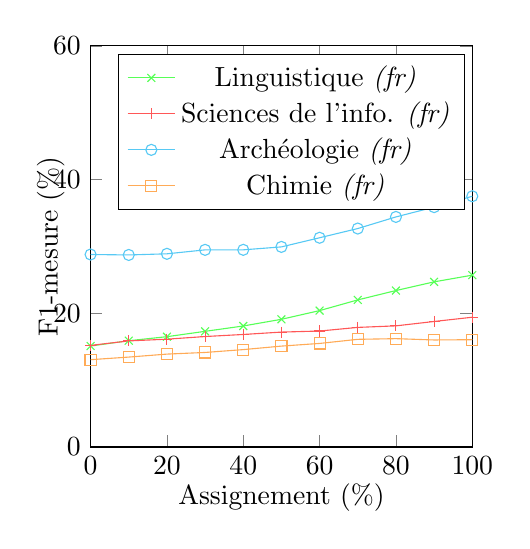
\begin{tikzpicture}
    \pgfkeys{/pgf/number format/.cd, fixed}
    \begin{axis}[x=0.0040\linewidth,
                 xtick={0, 20, ..., 100},
                 xmin=0,
                 xmax=100,
                 xlabel=Assignement (\%),
                 x label style={yshift=.34em},
                 y=0.007\linewidth,
                 ytick={0, 20, ..., 100},
                 ymin=0,
                 ymax=60,
                 ylabel=F1-mesure (\%),
                 y label style={yshift=-1.1em}]
      \addplot[green!66, mark=x] coordinates{
        (0, 15.1)
        (10, 15.9)
        (20, 16.5)
        (30, 17.3)
        (40, 18.1)
        (50, 19.1)
        (60, 20.4)
        (70, 22.0)
        (80, 23.4)
        (90, 24.7)
        (100, 25.7)
      };
      \addplot[red!66, mark=+] coordinates{
        (0, 15.1992)
        (10, 15.8659)
        (20, 16.1269)
        (30, 16.5223)
        (40, 16.8308)
        (50, 17.1875)
        (60, 17.3450)
        (70, 17.8887)
        (80, 18.1184)
        (90, 18.7733)
        (100, 19.4089)
      };
      \addplot[cyan!66, mark=o] coordinates{
        (0, 28.7887)
        (10, 28.7239)
        (20, 28.8927)
        (30, 29.4833)
        (40, 29.4880)
        (50, 29.9271)
        (60, 31.2943)
        (70, 32.6718)
        (80, 34.4101)
        (90, 35.8757)
        (100, 37.5003)
      };
      \addplot[orange!66, mark=square] coordinates{
        (0, 13.0605)
        (10, 13.4498)
        (20, 13.8944)
        (30, 14.1412)
        (40, 14.5673)
        (50, 15.0916)
        (60, 15.4902)
        (70, 16.1045)
        (80, 16.2055)
        (90, 16.0077)
        (100, 16.0506)
      };
      \legend{Linguistique \textit{(fr)}, Sciences de l'info. \textit{(fr)}, Archéologie \textit{(fr)}, Chimie \textit{(fr)}};
    \end{axis}
  \end{tikzpicture}
  \caption{Comportement de TopicCoRank en fonction du taux d'assignement
           \label{fig:assignment_variations}}
\end{figure}



        Enfin, nous réalisons une dernière expérience dans laquelle nous faisons
        varier la valeur du paramètre $\lambda$, qui détermine l'influence de la
        recommandation interne par rapport à la recommandation externe. Plus
        élevé est la valeur de $\lambda$, plus forte est l'influence de la
        recommandation interne et plus faible est l'influence de la
        recommentation externe. La figure~\ref{fig:lambda_variations_termith}
        montre le comportement de TopicCoRank lorsque nous faisons varier la
        valeur de $\lambda$ de 0 à 1 avec un pas de 0,1. Globalement,
        l'indexation par termes-clés est meilleure lorsque l'ordonnancement est
        fortement influencé par la recommandation externe que lorsqu'il ne
        l'est pas et utiliser une valeur de $\lambda$ qui assure l'équilibre
        entre l'influence interne et l'influence externe permet une performance
        quasi-optimale. Ces résultats montrent que notre choix de fixé $\lambda$
        à 0,5 est pertinent et nous conforte dans notre hypothèse qu'extraction
        et assignement doivent être réalisés conjointement.
        \begin{figure}[h!]
  \centering
  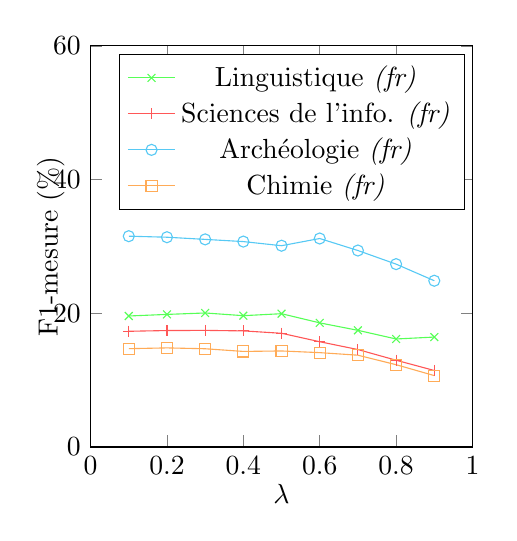
\begin{tikzpicture}
    \pgfkeys{/pgf/number format/.cd, fixed}
    \begin{axis}[x=0.4\linewidth,
                 xtick={0, 0.2, ..., 1.0},
                 xmin=0,
                 xmax=1.0,
                 xlabel=$\lambda$,
                 x label style={yshift=.34em},
                 y=0.007\linewidth,
                 ytick={0, 20, ..., 100},
                 ymin=0,
                 ymax=60,
                 ylabel=F1-mesure (\%),
                 y label style={yshift=-1.1em}]
      \addplot[green!66, mark=x] coordinates{
        (0.1, 19.5942)
        (0.2, 19.8314)
        (0.3, 20.0452)
        (0.4, 19.6420)
        (0.5, 19.9371)
        (0.6, 18.5649)
        (0.7, 17.4499)
        (0.8, 16.1558)
        (0.9, 16.4438)
      };
      \addplot[red!66, mark=+] coordinates{
        (0.1, 17.3100)
        (0.2, 17.4176)
        (0.3, 17.4420)
        (0.4, 17.3653)
        (0.5, 17.0094)
        (0.6, 15.7458)
        (0.7, 14.5758)
        (0.8, 12.9788)
        (0.9, 11.4421)
      };
      \addplot[cyan!66, mark=o] coordinates{
        (0.1, 31.5290)
        (0.2, 31.3748)
        (0.3, 31.0511)
        (0.4, 30.7214)
        (0.5, 30.1052)
        (0.6, 31.1819)
        (0.7, 29.3852)
        (0.8, 27.3498)
        (0.9, 24.8661)
      };
      \addplot[orange!66, mark=square] coordinates{
        (0.1, 14.7061)
        (0.2, 14.8227)
        (0.3, 14.6960)
        (0.4, 14.2947)
        (0.5, 14.3646)
        (0.6, 14.1136)
        (0.7, 13.7321)
        (0.8, 12.3091)
        (0.9, 10.6809)
      };
      \legend{Linguistique \textit{(fr)}, Sciences de l'info. \textit{(fr)}, Archéologie \textit{(fr)}, Chimie \textit{(fr)}};
    \end{axis}
  \end{tikzpicture}
  \caption{Comportement de TopicCoRank en fonction du taux d'assignement
           \label{fig:assignment_variations}}
\end{figure}


      
      \subsubsection{Évaluation de TopicCoRank hors domaines de spécialité}
      \label{subsubsec:main-domain_specific_keyphrase_annotation-supervised_automatic_keyphrase_annotation-evaluation-topiccorank_indepent_domains}
        \TODO{intro.}

        Le tableau~\ref{tab:topiccorank-comparison_results_general} montre les
        performances de TopicCoRank hors domaines de spécialités (\textsc{De}ft,
        SemEval et \textsc{Duc}) comparées à celles des méthodes de référence.
        Les résultats montrent de plus faibles performances qu'en domaines de
        spécialités. TopicCoRank échoue à améliorer TopicRank sur \textsc{De}ft,
        l'améliore légèrement sur SemEval et l'améliore significativement sur
        \textsc{Duc}, pour lequel nous utilisons des graphes de domaine très
        centrés sur le sujet d'actualité de chaque document de test.
        Contrairement à ce que nous observons en domaines de spécialités, c'est
        TopicCoRank qui est majoritairement le plus performant et c'est sa
        variantes TopicCoRank$_\textnormal{assign.}$ qui est la moins
        performante. Tout ceci s'explique par le fait que les termes-clés de
        référence de \textsc{De}ft et SemEval n'ont pas été produit à la manière
        de ceux des collections Termith. Ceux-ci sont fournis par les auteurs,
        pour \textsc{De}ft et par les auteurs et des lecteurs, pour SemEval.
        Aucun vocabulaire contrôlé n'est défini et les principes de conformité
        et d'homogénéité sur lesquels nous fondons nos hypothèses ne sont pas
        respectés. La contrainte de conformité n'étant pas respectée, la
        nécessité de l'assignement n'est pas garantie~; la contrainte
        d'homogénéité n'étant pas respectée non plus, le graphe de domaine que
        nous construisons contient des termes-clés de référence redondants et il
        faudrait, comme pour les termes-clés candidats, les grouper en sujets et
        définir une stratégie de sélection du terme-clé à assigner.
        \begin{table}
          \centering
          %\resizebox{\linewidth}{!}{
            \begin{tabular}{l|ccc|ccc|ccc}
              \toprule
              \multirow{2}{*}{\textbf{Méthode}} & \multicolumn{3}{c|}{\textbf{\textsc{De}ft}} & \multicolumn{3}{c|}{\textbf{\textsc{Duc}}} & \multicolumn{3}{c}{\textbf{SemEval}}\\
              \cline{2-10}
              & P & R & F & P & R & F & P & R & F\\
              \hline
              \textsc{Tf-Idf} & 10,4 & 19,1 & 13,3 & 24,9 & 32,1 & 27,7$^{~~}$ & 13,6 & $~~$9,3 & 10,9\\
              TopicRank & \textbf{11,9} & \textbf{21,5} & \textbf{14,9} & 17,9 & 23,7 & 20,1$^{~~}$ & 16,6 & 11,5 & 13,5\\
              KEA++ & --- & --- & --- & --- & --- & ---$^{~~}$ & --- & --- & ---\\
              \hline
              TopicCoRank$_\textnormal{extr.}$ & 10,1 & 19,1 & 13,0 & 24,6 & 35,5 & 27,2$^{~~}$ & 17,4 & 12,3 & 14,3\\
              TopicCoRank$_\textnormal{assign.}$ & $~~$6,8 & 12,8 & $~~$8,7 & 25,8 & 33,1 & 28,6$^{~~}$ & 11,8 & $~~$8,4 & $~~$9,7\\
              \hline
              TopicCoRank & $~~$8,7 & 16,2 & 11,2 & \textbf{28,2} & \textbf{36,3} & \textbf{31,3}$^\dagger$ & \textbf{17,6} & \textbf{12,5} & \textbf{14,5}\\
              \bottomrule
            \end{tabular}
          %}
        \caption[
          Résultat de l'extraction de dix termes-clés avec \textsc{Tf-Idf},
          TopicRank, \textsc{Kea++}, TopicCoRank$_\textnormal{\textit{extr.}}$,
          TopicCoRank$_\textnormal{\textit{assign.}}$ et TopicCoRank appliqués à
          \textsc{De}ft, SemEval et \textsc{Duc}
        ]{
          Résultat de l'extraction de dix termes-clés avec \textsc{Tf-Idf},
          TopicRank, \textsc{Kea++}, TopicCoRank$_\textnormal{\textit{extr.}}$,
          TopicCoRank$_\textnormal{\textit{assign.}}$ et TopicCoRank appliqués à
          \textsc{De}ft, SemEval et \textsc{Duc}. $\dagger$ indique une
          amélioration significative vis-à-vis des méthodes de référence, à
          0,001 pour le t-test de Student.
          \label{tab:topiccorank-comparison_results_general}}
        \end{table}

        La figure~\ref{fig:topiccorank-pr_curves_general} permet de comparer le
        comportement respectif des méthodes de référence, de TopicCoRank et de
        ses variantes, à l'aide de courbes rappel--précision. Contrairement aux
        domaines de spécialités, où TopicCoRank et ses variantes dominent les
        méthodes de référence, nous observons ici qu'aucune méthode dominante
        ne se dégage et, sauf sur \textsc{Duc}, il est difficile de statuer sur
        l'apport de TopicCoRank à TopicRank. Sur \textsc{De}ft, les courbes de
        TopicCoRank$_\textnormal{extr.}$ et TopicCoRank montrent aussi
        l'inconsistance des termes-clés de référence que nous évonquons
        au-dessus. Si TopicCoRank et ses variantes se démarquent largement sur
        les domaines de spécialités, ce n'est pas le cas sur des collections de
        données hors domaines de spécialités, dont l'indexation ne respecte pas
        les principes sur lesquels nos hypothèses sont fondées.
        \begin{figure}[h!]
  \subfigure[\textsc{De}ft \textit{(fr)}]{
    \begin{tikzpicture}
      \pgfkeys{/pgf/number format/.cd, fixed}
      \begin{axis}[x=0.0057\linewidth,
                   xtick={0, 20, 40, ..., 100},
                   xmin=0,
                   xmax=60,
                   xlabel=rappel (\%),
                   x label style={yshift=.34em},
                   y=0.0057\linewidth,
                   ytick={0, 20, ..., 100},
                   ymin=0,
                   ymax=60,
                   ylabel=précision (\%),
                   y label style={yshift=-1.1em}]
        \addplot [green!66, mark=x] file {input/figure/data/deft_tfidf.csv};
        \addplot [red!66, mark=+] file {input/figure/data/deft_topicrank.csv};
        \addplot [orange!66, mark=square] file {input/figure/data/deft_topiccorank_extr.csv};
        \addplot [black!66, mark=triangle] file {input/figure/data/deft_topiccorank_assign.csv};
        \addplot [gray!66, mark=diamond] file {input/figure/data/deft_topiccorank.csv};
        %%%%%%%%%%%%%%%%%%%%%%%%%%%%%%%%%%%%%%%%%%%%%%%%%%%%%%%%%%%%%%%%%%%%%%%%
        \addplot [dotted, domain=35:100] {(50 * x) / ((2 * x) - 50)};
        \addplot [dotted, domain=25:100] {(40 * x) / ((2 * x) - 40)};
        \addplot [dotted, domain=15:100] {(30 * x) / ((2 * x) - 30)};
        \addplot [dotted, domain=10:100] {(20 * x) / ((2 * x) - 20)};
        \addplot [dotted, domain=5:100] {(10 * x) / ((2 * x) - 10)};
      \end{axis}
      \node at (4.85,3.6) [anchor=east] {\footnotesize{F=50,0}};
      \node at (4.85,2.6) [anchor=east] {\footnotesize{F=40,0}};
      \node at (4.85,1.8) [anchor=east] {\footnotesize{F=30,0}};
      \node at (4.85,1.15) [anchor=east] {\footnotesize{F=20,0}};
      \node at (4.85,0.6) [anchor=east] {\footnotesize{F=10,0}};
    \end{tikzpicture}
  }
  \subfigure[Semeval \textit{(en)}]{
    \begin{tikzpicture}
      \pgfkeys{/pgf/number format/.cd, fixed}
      \begin{axis}[x=0.0057\linewidth,
                   xtick={0, 20, 40, ..., 100},
                   xmin=0,
                   xmax=60,
                   xlabel=rappel (\%),
                   x label style={yshift=.34em},
                   y=0.0057\linewidth,
                   ytick={0, 20, ..., 100},
                   ymin=0,
                   ymax=60,
                   ylabel=précision (\%),
                   y label style={yshift=-1.1em}]
        \addplot [green!66, mark=x] file {input/figure/data/semeval_tfidf.csv};
        \addplot [red!66, mark=+] file {input/figure/data/semeval_topicrank.csv};
        \addplot [orange!66, mark=square] file {input/figure/data/semeval_topiccorank_extr.csv};
        \addplot [black!66, mark=triangle] file {input/figure/data/semeval_topiccorank_assign.csv};
        \addplot [gray!66, mark=diamond] file {input/figure/data/semeval_topiccorank.csv};
        %%%%%%%%%%%%%%%%%%%%%%%%%%%%%%%%%%%%%%%%%%%%%%%%%%%%%%%%%%%%%%%%%%%%%%%%
        %\addplot [dotted, domain=35:100] {(50 * x) / ((2 * x) - 50)};
        %\addplot [dotted, domain=25:100] {(40 * x) / ((2 * x) - 40)};
        \addplot [dotted, domain=15:100] {(30 * x) / ((2 * x) - 30)};
        \addplot [dotted, domain=10:100] {(20 * x) / ((2 * x) - 20)};
        \addplot [dotted, domain=5:100] {(10 * x) / ((2 * x) - 10)};
        %%%%%%%%%%%%%%%%%%%%%%%%%%%%%%%%%%%%%%%%%%%%%%%%%%%%%%%%%%%%%%%%%%%%%%%%
        \legend{\textsc{Tf-Idf}, TopicRank, TopicCoRank$_\textnormal{extr.}$,
                TopicCoRank$_\textnormal{assign.}$, TopicCoRank};        
      \end{axis}
      %\node at (4.85,3.6) [anchor=east] {\footnotesize{F=50,0}};
      %\node at (4.85,2.6) [anchor=east] {\footnotesize{F=40,0}};
      \node at (4.85,1.8) [anchor=east] {\footnotesize{F=30,0}};
      \node at (4.85,1.15) [anchor=east] {\footnotesize{F=20,0}};
      \node at (4.85,0.6) [anchor=east] {\footnotesize{F=10,0}};
    \end{tikzpicture}
  }
  \subfigure[\textsc{Duc} \textit{(en)}]{
    \begin{tikzpicture}
      \pgfkeys{/pgf/number format/.cd, fixed}
      \begin{axis}[x=0.0057\linewidth,
                   xtick={0, 20, 40, ..., 100},
                   xmin=0,
                   xmax=60,
                   xlabel=rappel (\%),
                   x label style={yshift=.34em},
                   y=0.0057\linewidth,
                   ytick={0, 20, ..., 100},
                   ymin=0,
                   ymax=60,
                   ylabel=précision (\%),
                   y label style={yshift=-1.1em}]
        \addplot [green!66, mark=x] file {input/figure/data/duc_tfidf.csv};
        \addplot [red!66, mark=+] file {input/figure/data/duc_topicrank.csv};
        \addplot [orange!66, mark=square] file {input/figure/data/duc_topiccorank_extr.csv};
        \addplot [black!66, mark=triangle] file {input/figure/data/duc_topiccorank_assign.csv};
        \addplot [gray!66, mark=diamond] file {input/figure/data/duc_topiccorank.csv};
        %%%%%%%%%%%%%%%%%%%%%%%%%%%%%%%%%%%%%%%%%%%%%%%%%%%%%%%%%%%%%%%%%%%%%%%%
        \addplot [dotted, domain=35:100] {(50 * x) / ((2 * x) - 50)};
        \addplot [dotted, domain=25:100] {(40 * x) / ((2 * x) - 40)};
        \addplot [dotted, domain=15:100] {(30 * x) / ((2 * x) - 30)};
        \addplot [dotted, domain=10:100] {(20 * x) / ((2 * x) - 20)};
        \addplot [dotted, domain=5:100] {(10 * x) / ((2 * x) - 10)};
      \end{axis}
      \node at (4.85,3.6) [anchor=east] {\footnotesize{F=50,0}};
      \node at (4.85,2.6) [anchor=east] {\footnotesize{F=40,0}};
      \node at (4.85,1.8) [anchor=east] {\footnotesize{F=30,0}};
      \node at (4.85,1.15) [anchor=east] {\footnotesize{F=20,0}};
      \node at (4.85,0.6) [anchor=east] {\footnotesize{F=10,0}};
    \end{tikzpicture}
  }
  \caption{Courbes de rappel-précision de \textsc{Tf-Idf}, TopicRank,
           TopicCoRank$_\textnormal{extr.}$, TopicCoRank$_\textnormal{assign.}$
           et TopicCoRank appliqués à \textsc{De}ft, SemEval et \textsc{Duc}
           \label{fig:topiccorank-pr_curves}}
\end{figure}



        Comme pour l'évaluation en domaines de spécialités, le
        tableau~\ref{tab:assignment_ratio_general} reporte les taux d'extraction
        et d'assignement réalisés par TopicCoRank sur \textsc{De}ft, SemEval et
        \textsc{Duc}. Ceux-ci montrent aussi que les deux catégories
        d'indexation sont réalisées conjointement, cette fois-ci sans
        prédominance de l'une face à l'autre.
        \begin{table}[h]
          \centering
          \begin{tabular}{l|c|c}
              \toprule
              & Extraction (\%) & Assignement (\%)\\
              \hline
              \textsc{De}ft \textit{(fr)} & 48,4 & 51,6\\
              SemEval \textit{(en)} & 61,4 & 38,6\\
              \textsc{Duc} \textit{(en)} & 46,9 & 53,1\\
              \bottomrule
          \end{tabular}
          \caption{Taux moyens d'extraction et d'assignement réalisés par
                   TopicCoRank pour les collections Termith
                   \label{tab:assignment_ratio_general}}
        \end{table}

        La figure~\ref{fig:assignment_variations_termith} montrent les
        performances de TopicCoRank lorsque nous forçons le taux d'assignement,
        de 0~\% à 100~\% avec un pas de 10~\%. Contrairement à la courbe de
        performances en domaines de spécialités, celle de TopicCoRank hors
        domaines de spécialités est croissante puis décroissante pour \text{Duc}
        et décroissante pour \textsc{De}ft et SemEval. Cela signifie que
        l'ordonnancement des termes-clés de référence est moins efficace hors
        domaines de spécialités qu'en domaines de spécialités. Il est toutefois
        intéressant de noter que la courbe de performance de \textsc{Duc} montre
        que le taux d'assignement effectué par TopicCoRank sans que nous le
        forçions est le taux permettant la performance optimale. Sur
        \textsc{Duc}, les performances de TopicCoRank sont les meilleures qu'il
        puisse obtenir.
        \begin{figure}[h!]
  \centering
  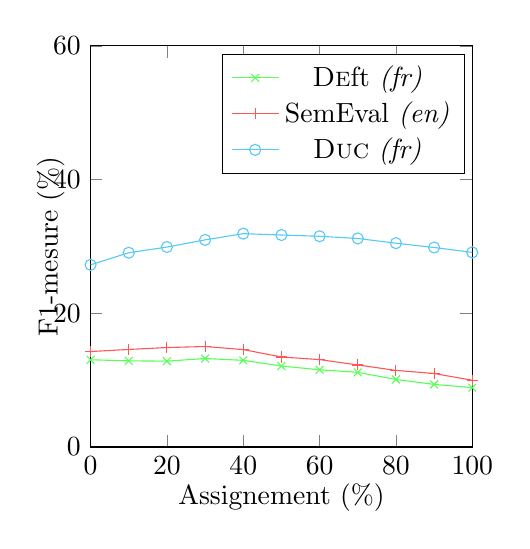
\begin{tikzpicture}
    \pgfkeys{/pgf/number format/.cd, fixed}
    \begin{axis}[x=0.0040\linewidth,
                 xtick={0, 20, ..., 100},
                 xmin=0,
                 xmax=100,
                 xlabel=Assignement (\%),
                 x label style={yshift=.34em},
                 y=0.007\linewidth,
                 ytick={0, 20, ..., 100},
                 ymin=0,
                 ymax=60,
                 ylabel=F1-mesure (\%),
                 y label style={yshift=-1.1em}]
      \addplot[green!66, mark=x] coordinates{
        (0, 13.0470)
        (10, 12.8868)
        (20, 12.8409)
        (30, 13.2342)
        (40, 12.9643)
        (50, 12.1117)
        (60, 11.5492)
        (70, 11.1649)
        (80, 10.1043)
        (90, 9.3643)
        (100, 8.8794)
      };
      \addplot[red!66, mark=+] coordinates{
        (0, 14.2790)
        (10, 14.5905)
        (20, 14.8776)
        (30, 15.0293)
        (40, 14.5713)
        (50, 13.4616)
        (60, 13.0731)
        (70, 12.2721)
        (80, 11.4582)
        (90, 10.9929)
        (100, 9.9841)
      };
      \addplot[cyan!66, mark=o] coordinates{
        (0, 27.2447)
        (10, 29.0553)
        (20, 29.9039)
        (30, 30.9763)
        (40, 31.9071)
        (50, 31.7050)
        (60, 31.5150)
        (70, 31.1887)
        (80, 30.4816)
        (90, 29.8382)
        (100, 29.1068)
      };
      \legend{\textsc{De}ft \textit{(fr)}, SemEval \textit{(en)}, \textsc{Duc} \textit{(fr)}};
    \end{axis}
  \end{tikzpicture}
  \caption{Comportement de TopicCoRank en fonction du taux d'assignement
           \label{fig:assignment_variations}}
\end{figure}



        Enfin, nous réalisons une dernière expérience dans laquelle nous faisons
        aussi varier la valeur du paramètre $\lambda$ pour déterminer si
        équilibrer l'influence de la recommandation interne et de la
        recommandation externe est une solution générique et pour vérifier si
        TopicCoRank tire effectivement profit des deux graphes. La
        figure~\ref{fig:lambda_variations_general}
        montre le comportement de TopicCoRank lorsque nous faisons varier la
        valeur de $\lambda$ de 0 à 1 avec un pas de 0,1. Sur \textsc{Duc}, comme
        en domaines des spécialités, l'indexation par termes-clés est meilleure
        lorsque l'ordonnancement est fortement influencé par la recommandation
        externe que lorsqu'il ne l'est pas. Sur \textsc{De}ft et SemEval, c'est
        l'inverse~: l'indexation par termes-clés est plus performante lorsque
        l'ordonnancement au sein de chaque graphe n'est que très faiblement
        influencé par l'ordonnancement au sein de l'autre. Toutefois, lorsque
        $\lambda$ est au voisinage de sa valeur définie par défaut, nous
        observons un compromis. Comme en domaines de spécialités, ces résultats
        montrent que notre choix de fixé $\lambda$ à 0,5 est pertinent.
        \begin{figure}[t]
  \centering
  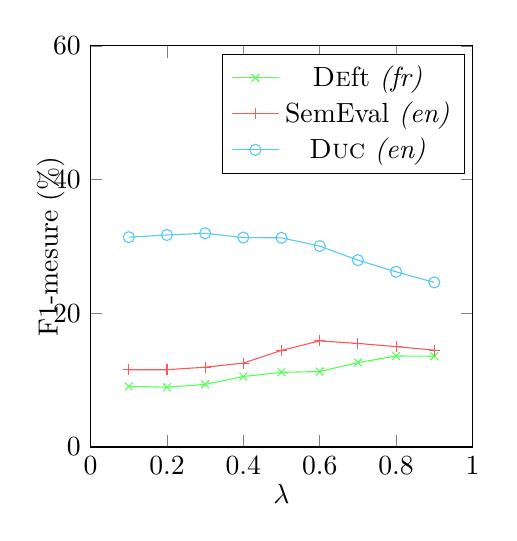
\begin{tikzpicture}
    \pgfkeys{/pgf/number format/.cd, fixed}
    \begin{axis}[x=0.4\linewidth,
                 xtick={0, 0.2, ..., 1.0},
                 xmin=0,
                 xmax=1.0,
                 xlabel=$\lambda$,
                 x label style={yshift=.34em},
                 y=0.007\linewidth,
                 ytick={0, 20, ..., 100},
                 ymin=0,
                 ymax=60,
                 ylabel=F1-mesure (\%),
                 y label style={yshift=-1.1em}]
      \addplot[green!66, mark=x] coordinates{
        (0.1, 9.0736)
        (0.2, 8.9392)
        (0.3, 9.3693)
        (0.4, 10.5436)
        (0.5, 11.1626)
        (0.6, 11.2902)
        (0.7, 12.6269)
        (0.8, 13.6109)
        (0.9, 13.5765)
      };
      \addplot[red!66, mark=+] coordinates{
        (0.1, 11.5509)
        (0.2, 11.5618)
        (0.3, 11.9382)
        (0.4, 12.5558)
        (0.5, 14.4539)
        (0.6, 15.8712)
        (0.7, 15.4920)
        (0.8, 15.0102)
        (0.9, 14.4863)
      };
      \addplot[cyan!66, mark=o] coordinates{
        (0.1, 31.3789)
        (0.2, 31.7112)
        (0.3, 31.9601)
        (0.4, 31.3222)
        (0.5, 31.2842)
        (0.6, 30.0481)
        (0.7, 27.9426)
        (0.8, 26.1973)
        (0.9, 24.6206)
      };
      \legend{\textsc{De}ft \textit{(fr)}, SemEval \textit{(en)}, \textsc{Duc} \textit{(en)}};
    \end{axis}
  \end{tikzpicture}
  \caption{Performance de TopicCoRank, appliqué à \textsc{De}ft, SemEval et
           \textsc{Duc}, lorsque le paramètre $\lambda$ varie
           \label{fig:lambda_variations_general}}
\end{figure}



    \subsection{Analyse d'erreurs}
    \label{subsec:main-domain_specific_keyphrase_annotation-supervised_automatic_keyphrase_annotation-error_analysis}
      Dans cette section, nous nous intéressons aux termes-clés issus du graphe
      représentatif du domaine. Nous analysons les termes-clés corrects et
      incorrects obtenus par assignement.\TODO{\dots}

      \subsubsection{Analyse des vrais positifs}
      \label{subsec:main-domain_specific_keyphrase_annotation-supervised_automatic_keyphrase_annotation-error_analysis-true_positives}

      \subsubsection{Analyse des faux positifs}
      \label{subsec:main-domain_specific_keyphrase_annotation-supervised_automatic_keyphrase_annotation-error_analysis-false_positives}

    \subsection{Bilan}
    \label{subsec:main-domain_specific_keyphrase_annotation-supervised_automatic_keyphrase_annotation-conclusion}
      Avec TopicCoRank, nous proposons une extension de la méthode TopicRank,
      que nous présentons dans la
      section~\ref{sec:main-domain_specific_keyphrase_annotation-unsupervised_automatic_keyphrase_extraction}
      (page~\pageref{sec:main-domain_specific_keyphrase_annotation-unsupervised_automatic_keyphrase_extraction}).
      Cette extension apporte à TopicRank la capacité à assigner des
      termes-clés, soit à réaliser la tâche d'indexation par termes-clés dans sa
      globalité. Pour ce faire, TopicCoRank utilise les termes-clés de
      références des documents d'entraînement comme vocabulaire contrôlé, crée
      un graphe dont chaque n\oe{}uds est une entrée du vocabulaire connecté aux
      autres lorsqu'ils sont termes-clés d'un même document, puis unifie se
      graphe au graphe de sujets de TopicRank.

      \TODO{domaines de spécialité Vs. cas général}

  %-----------------------------------------------------------------------------

  \section{Évaluation manuelle en domaines de spécialités}
  \label{sec:main-domain_specific_keyphrase_annotation-manual_evaluation}
    Pour évaluer les performances d'une méthode d'indexation automatique par
    termes-clés et la comparer aux autres méthodes, il est courant d'utiliser un
    système d'évaluation automatique. Un tel système utilise un jugement de
    référence qu'il compare aux sorties de la méthode
    automatique~\cite{voorhees2002philosophy}. Dans le cas de l'indexation par
    termes-clés, si un terme-clé donné par la méthode fait partie des
    termes-clés de référence (jugement de référence), alors celui-ci est jugé
    correct, sinon il est jugé incorrect. Alternative viable et plus accessible
    que l'évaluation manuelle, l'évaluation automatique possède toutefois un
    inconvénient majeur~: la condition stricte d'appartenance au jugement de
    référence n'est pas adaptée à une tâche subjective telle que celle de
    l'indexation par termes-clés et elle rend donc pessimiste l'évaluation de
    cette dernière. En effet, un même sujet peut êrte représenté par plusieurs
    expressions synonymiques, mais le jugement de référence n'en accepte qu'une
    seule alors que les autres peuvent aussi
    convenir~\cite{hasan2014state_of_the_art}. Certains travaux tentent de
    résoudre ce problème en acceptant des variantes des termes-clés de
    référence~\cite{zesch2009rprecision,kim2010rprecision}. Cependant, aucun ne
    quantifie la divergence sémantique entre un terme-clé de référence et sa
    supposée variante. De cette ménière, l'évaluation pert certes en pessimisme,
    mais aussi en exactitude.
    
    Pour compléter les évaluations automatiques que nous réalisons pour évaluer
    nos travaux, le projet Termith et l'Inist mettent à notre disposition des
    indexeurs professionnels pour évaluer manuellement les termes-clés produits
    par nos méthodes, pour les domaines de la linguistique, des sciences de
    l'information, de l'archéologie et de la chimie (ressource Termith).

    \subsection{Protocole d'évaluation manuelle}
    \label{subsec:main-automatic_evaluation_of_keyphrase_annotation-methodology-evaluation_protocol}
      L'évaluation manuelle concerne dix termes-clés extraits et/ou assignés par
      chaque méthode d'indexation par termes-clés. Le protocole que nous
      proposons permet d'évaluer deux aspects de l'indexation automatique par
      termes-clés~:
      \begin{enumerate}
        \item{Pertinence~: chaque terme-clé fourni par la méthode d'indexation
              automatique par termes-clés est-il important pour la compréhension
              du contenu principal du document~?}
        \item{Silence~: quel est le degré d'importance des informations perdues
              entre les termes-clés de référence et les termes-clés fournis par
              la méthode d'indexation automatique par termes-clés~?}
      \end{enumerate}
      L'évaluation de la pertinence traite le même aspect que l'évaluation
      automatique~: le nombre de termes-clés corrects doit être maximisé pour
      obtenir la meilleure performance. L'évaluation du silence traite un aspect
      qui n'est pas traité par l'évaluation automatique. Elle a une dimension
      plus sémantique~: les termes-clés corrects dont l'information est la plus
      capitale à la compréhension du contenu principal du document doivent être
      priorisés pour obtenir la meilleure performance.

      Afin de minimiser les problèmes d'ambiguïté et de subjectivité de certains
      cas de figure, la pertinence et le silence sont évalués sur une échelle à
      trois valeurs~: une valeur représentant l'échec, une autre représentant le
      succès et une dernière valeur représentant un cas intermédiaire.

      \subsubsection{Évaluation de la pertinence}
      \label{subsubsec:main-automatic_evaluation_of_keyphrase_annotation-methodology-evaluation_protocol-relevancy}
        \TODO{expliquer que l'indexeur ne peut pas voir les termes-clés inist
        lors de cette évaluation}
        Pour évaluer la pertinence d'un terme-clé fourni par une méthode
        d'indexation par termes-clés, l'évaluateur doit lui attribuer un score
        sur une échelle de 0 à 2. Ce score distingue les termes-clés incorrects
        (0), les termes-clés corrects (2) et les variantes de ces derniers (1).

        Pour permettre une étude précise de cette évaluation, les indexeurs
        professionnels doivent indiquer la forme préférée des termes-clés
        auquels ils donnent un score de 1 (variantes). Une variante peut faire
        référence à deux catégories de formes préférées, qui induisent deux
        raisonnements différents~:
        \begin{itemize}
          \item{variante d'un terme-clé déjà fourni (score de
                2)~$\Rightarrow$~la méthode d'indexation par termes-clés fourni
                des termes-clés redondants~;}
          \item{variante d'un terme-clé non fourni mais présent dans le
              texte~$\Rightarrow$~la méthode d'indexation par termes-clés
                identifie correctement les sujets importants du document, mais
                peine à trouver leur forme la plus appropriée pour les
                représenter.}
        \end{itemize}

        Lorsque la forme préférée n'est pas présente dans le document, nous
        estimons que la méthode d'indexation a fourni un terme-clé correct,
        auquel cas il se voit attribuer le score de 2. Les formes variantes
        résultant d'un accord en nombre (pluriel) obtiennent aussi un score de
        2, lorsque la forme normalisée (singulier) ne se trouve pas parmi les
        termes-clés fournis.

      \subsubsection{Évaluation du silence}
      \label{subsubsec:main-automatic_evaluation_of_keyphrase_annotation-methodology-evaluation_protocol-silence}
        \TODO{explique que l'évaluateur effectue cette évaluation après la
        pertinence et qu'il ne peut pas revenir à la pertinence car ça
        introduirait un biais}
        Pour évaluer le silence, l'évaluateur doit attribuer à chaque terme-clé
        de référence un score indiquant le degré d'importance de l'information
        qu'il véhicule et qui n'est pas capturée par les termes-clés fournis par
        une méthode d'indexation par termes-clés. Sur une échelle de 0 à 2, ce
        score permet d'indiquer s'il n'y pas de perte d'information (0), si
        l'information perdue est capitale (2) ou si elle est secondaire (1).
        Lorsqu'un terme-clé de référence obtient un score de 0, cela signifie
        soit qu'il fait partie des termes-clés fournis par la méthode
        d'indexation par termes-clés, soit que l'indexeur juge qu'il ne devrait
        pas être un terme-clé de référence, c'est-à-dire que c'est une erreur
        parmi les termes-clés de référence.

        Une perte d'information est jugée secondaire (score de 1) dans deux
        cas de figure différents~:
        \begin{itemize}
          \item{terme-clé de référence secondaire~: le terme-clé de référence
                n'apporte pas l'information la plus importante~;}
          \item{terme-clé de référence générique~: le terme-clé de référence
                n'est pas suffisamment spécifique au contenu du document, il a
                un usage classificatoire~;}
        \end{itemize}
        Afin de minimiser les pertes d'informations dues à des termes-clés de
        référence qui ne sont pas présents dans le document, les évaluateurs
        leur attribuent un score de 1.

    \subsection{Évaluation manuelle des méthodes proposées}
    \label{subsec:main-domain_specific_keyphrase_annotation-manual_evaluation-analysis}
      Dans cette section, nous analysons l'évaluation manuelle de TopicRank,
      TopicCoRank, d'une méthode de référence non supervisée, \textsc{Tf-Idf},
      et d'une méthode de référence supervisée, \textsc{Kea}. L'évaluation est
      effectuée par un indexeur professionnel par document.

      Dans un premier temps, nous analysons l'évaluation manuelle de TopicRank
      et la comparons à celle de \textsc{Tf-Idf}, puis, dans un second temps,
      nous analysons l'évaluation manuelle de TopicCoRank et la comparons à
      celle de \textsc{Kea}.

      \subsubsection{Analyse de TopicRank}
      \label{subsubsec:main-domain_specific_keyphrase_annotation-manual_evaluation-analysis-topicrank}
        \TODO{\dots}
      
        ~\\Le
        tableau~\ref{tab:main-automatic_evaluation_of_keyphrase_annotation-results-topicrank-pertinence_score_ratio}
        dresse le bilan des scores de pertinence attribués en moyenne par
        méthode. Pour le score de 1, qui indique qu'un terme-clé est un forme
        variante, nous distinguons le cas où la variante est redondante du cas
        où la variante n'est pas redondante. Globalement, nous observons que
        TopicRank est meilleur que \textsc{Tf-Idf}. TopicRank fournit plus de
        termes-clés pertinents que \textsc{Tf-Idf}, mais fait aussi plus
        d'erreurs. Les termes-clés ayant un score de 1 donnent un explication
        intéressante à cette contradiction. En effet, \textsc{Tf-Idf} à une
        forte tendence à extraire des termes-clés redondant, soit des
        termes-clés variantes de termes-clés déjà extrait. En revanche,
        TopicRank remplit presque son objectif de ne pas extraire de termes-clés
        redondant, avec seulement 0,9~\% de termes-clés redondants. Comme nous
        l'avons aussi observé lors de l'évaluation automatique de TopicRank (cf
        section~\ref{subsec:main-automatic_keyphrase_annotation-unsupervised_automatic_keyphrase_extraction-evaluation}
        page~\ref{subsec:main-automatic_keyphrase_annotation-unsupervised_automatic_keyphrase_extraction-evaluation}),
        celui-ci extrait cependant plus de termes-clés variantes non redondants,
        c'est-à-dire que la strategie de TopicRank pour sélectionner le meilleur
        terme-clé pour un sujet n'est pas optimale.
        \begin{table}[h!]
          \centering
          \begin{tabular}{l|c|c|c|c}
            \toprule
            \multirow{2}{*}{\textbf{Méthode}} & \multirow{2}{*}{\textbf{0}} & \multicolumn{2}{c|}{\textbf{1}} & \multirow{2}{*}{\textbf{2}}\\
            \cline{3-4}
            & & \multicolumn{1}{p{.175\linewidth}|}{\centering{}redondant} & \multicolumn{1}{p{.175\linewidth}|}{\centering{}non redondant} &\\
            \hline
            \textsc{Tf-Idf} & \textbf{53,8~\%} & 6,8~\% & 4,2~\% & 35,3~\%\\
            TopicRank & 56,3~\% & \textbf{0,9~\%} & \textbf{5,7~\%} & \textbf{37,1~\%}\\
            \bottomrule
          \end{tabular}
          \caption{Taux de termes-clés avec un score de 0, de 1 ou de 2 pour
                   l'évaluation de la pertinence de \textsc{Tf-Idf} et de
                   TopicRank
                   \label{tab:main-automatic_evaluation_of_keyphrase_annotation-results-topicrank-pertinence_score_ratio}}
        \end{table}

        Le
        tableau~\ref{tab:main-automatic_evaluation_of_keyphrase_annotation-results-topicrank-prf}
        présente les performances de \textsc{Tf-Idf} et de TopicRank, en termes
        de précision, de rappel et de f-mesure, et les compare à celles
        observées par notre système d'évaluation automatique. Pour calculer ces
        performances, les termes-clés ayant un score de 2 sont considérés
        corrects, de même que ceux ayant un score de 1 non redondants. La
        difficulté d'évaluer automatiquement la tâche d'indexation par
        termes-clés se confirme. Les conclusions ne sont pas les mêmes, puisque
        de manière automatique TopicRank est moins performant que
        \textsc{Tf-Idf} alors qu'il est plus permformant selon l'évaluation
        manuelle. Nous observons aussi des différences d'environ 30 points entre
        les mesures obtenues manuellement et automatiquement. Les résultats
        montrent ici que la tâche d'indexation par termes-clés est effectivement
        subjective et que l'évaluation manuelle permet de réduire ce problème.
        \begin{table}[h!]
          \centering
          \begin{tabular}{l|ccc|ccc}
            \toprule
            \multirow{2}{*}{\textbf{Méthode}} & \multicolumn{3}{c|}{\textbf{Manuel}} & \multicolumn{3}{c}{\textbf{Automatique}}\\
            \cline{2-7}
            & P & R & F & P & R & F\\
            \hline
            \textsc{Tf-Idf} & 39,5 & 29,7 & 33,5 & \textbf{13,0} & \textbf{15,4} & \textbf{13,9}\\
            TopicRank & \textbf{42,8} & \textbf{32,2} & \textbf{36,2} & 11,2 & 13,1 & 11,9\\
            \bottomrule
          \end{tabular}
          \caption[
            Performances de \textsc{Tf-Idf} et de TopicRank en termes de
            précision, de rappel et de f-mesure
          ]{
            Performances de \textsc{Tf-Idf} et de TopicRank en termes de
            précision (P), de rappel (R) et de f-mesure (F)
            \label{tab:main-automatic_evaluation_of_keyphrase_annotation-results-topicrank-prf}}
        \end{table}
      
        ~\\Le
        tableau~\ref{tab:main-automatic_evaluation_of_keyphrase_annotation-results-topicrank-silence_score_ratio}
        dresse le bilan des scores de silence attribués en moyenne par méthode.
        D'après la description donnée pour chacun des scores, la méthode qui
        capture le plus d'informations est celle qui maximise le nombre de
        termes-clés de référence ayant un score de silence 0 et qui minimise
        ceux ayant un score de 1 et de 2. De ce fait, nous observons que
        TopicRank couvre mieux le contenu principal des documents que
        \textsc{Tf-Idf}.
        \begin{table}[h!]
          \centering
          \begin{tabular}{l|c|c|c}
            \toprule
            \textbf{Méthode} & \textbf{0} & \textbf{1} & \textbf{2}\\
            \hline
            \textsc{Tf-Idf} & 31,4~\% & 48,5~\% & 20,1~\%\\
            TopicRank & \textbf{35,0~\%} & \textbf{48,3~\%} & \textbf{16,8~\%}\\
            \bottomrule
          \end{tabular}
          \caption{Taux de termes-clés de référence avec un score de 0, de 1 ou
                   de 2 pour l'évaluation du silence de \textsc{Tf-Idf} et de
                   TopicRank
                   \label{tab:main-automatic_evaluation_of_keyphrase_annotation-results-topicrank-silence_score_ratio}}
        \end{table}

      \subsubsection{Analyse de TopicCoRank}
      \label{subsubsec:main-domain_specific_keyphrase_annotation-manual_evaluation-analysis-topiccorank}
        \TODO{\dots}

    \subsection{Bilan}
    \label{subsec:main-domain_specific_keyphrase_annotation-manual_evaluation-conclusion}
      \TODO{mettre en évidence les points forts et les faiblesses}

      \TODO{L'évaluation manuelle de TopicRank, et sa comparaison avec
      \textsc{Tf-Idf}, montre l'apport de TopicRank vis-à-vis de l'état de
      l'art. Les résultats montrent aussi que TopicRank remplit effectivement
      l'objectif d'éviter l'extraction de termes-clés redondants.}

  %-----------------------------------------------------------------------------

  \section{Conclusion}
  \label{sec:main-domain_specific_keyphrase_annotation-conclusion}
    \TODO{\dots}

